% !TEX root = ../main.tex
\paragraph{Drift Chambers (DC)}
    The forward tracking system in the experiment consists of three independent drift chambers in each of the six sectors of the torus magnet.
    These drift chambers serve as the primary tracking detectors and are supported by the six coils of the torus magnet.

    Each sector of the torus magnet contains a total of 36 layers in the drift chambers, with each layer having 112 sense wires.
    The sense wires are arranged in three regions, with each region comprising twelve layers.
    This configuration results in a total of 112 x 36 sense wires per sector.

    \begin{wrapfigure}{r}{0.50\textwidth}
        \frame{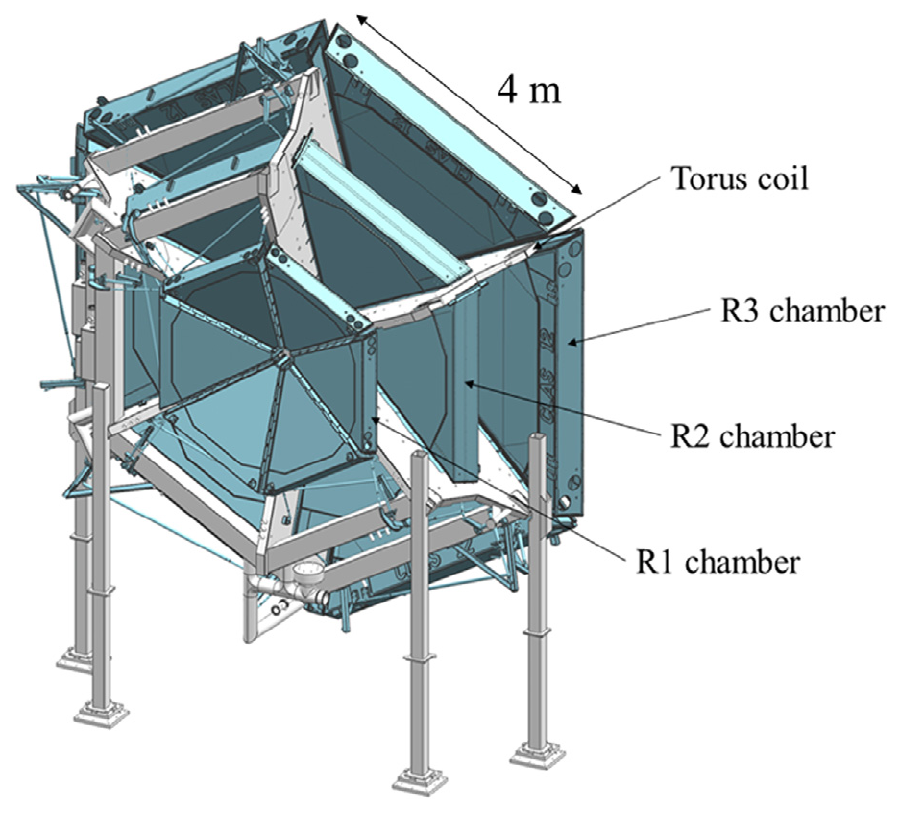
\includegraphics[width=\linewidth]{212dc.png}}
        \caption[DC]
        {Drift Chambers (DC) render.
        Each of the DC regions are denoted as R1, R2, and R3 in the figure.}
        \floatfoot{Source: \href{https://jlab.org/physics/hall-b/clas12}{CLAS12 wiki}.}
        \label{fig::11.212::dc}
    \end{wrapfigure}

    The arrangement of the drift chambers around the torus coil can be visualised in Figure \ref{fig::11.212::dc}.
    The figure shows the positioning of the three regions of the drift chambers in each sector of the torus magnet.

    In terms of location, the first region of the drift chambers is situated at the entrance to the torus magnetic field region.
    The second region is positioned inside the magnet, where the magnetic field is close to its maximum strength.
    Finally, the third region is located downstream of the torus magnet, in a low magnetic field space.

    This arrangement of the drift chambers around the torus magnet provides independent and redundant tracking capabilities in each of the six torus sectors.
    It allows for precise reconstruction of charged particle trajectories and momentum measurements in the experiment.

    Each of the three regions in the drift chambers consists of six "superlayers," where each superlayer comprises two layers.
    The wires in one layer are strung at a stereo angle of $+6\degree$ relative to the sector midplane, while the wires in the other layer are strung at a stereo angle of $-6\degree$.
    This stereo configuration provides excellent resolution in the polar angle ($\Delta\theta < 2 ~\text{mrad}$) and good resolution in the azimuthal scattering angle ($\Delta\phi < 2 ~\text{mrad}$).

    \begin{wrapfigure}{l}{0.50\textwidth}
        \frame{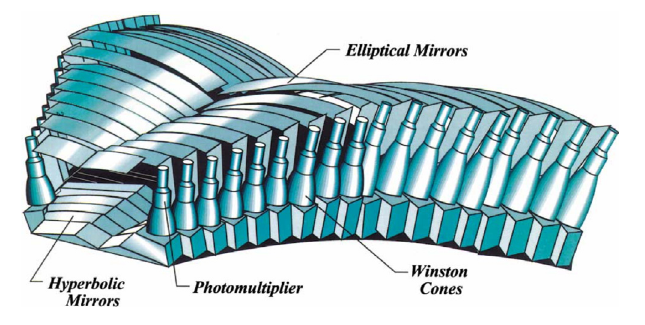
\includegraphics[width=\linewidth]{213ltcc.png}}
        \caption[LTCC Mirror System]
        {Layout and components of the optical mirror system within each LTCC box from the design model.}
        \floatfoot{Source: \href{https://jlab.org/physics/hall-b/clas12}{CLAS12 wiki}.}
        \label{fig::11.213::ltcc}
    \end{wrapfigure}

    The drift chambers are capable of detecting ionising particles with momenta above $200 ~\text{MeV}/\text{c}$, with a momentum resolution of $\Delta p/p$ less than $0.5\%$. This level of resolution corresponds to a track momentum resolution of $3\%$ to $5\%$.
    The high precision in momentum measurements allows for accurate reconstruction of particle trajectories and precise determination of their momenta, which is crucial for the physics analysis in the experiment \cite{mestayer2020}.
